\let\negmedspace\undefined
\let\negthickspace\undefined
\documentclass[journal]{IEEEtran}
\usepackage[a5paper, margin=10mm, onecolumn]{geometry}
%\usepackage{lmodern} % Ensure lmodern is loaded for pdflatex
\usepackage{tfrupee} % Include tfrupee package

\setlength{\headheight}{1cm} % Set the height of the header box
\setlength{\headsep}{0mm}     % Set the distance between the header box and the top of the text

\usepackage{gvv-book}
\usepackage{gvv}
\usepackage{cite}
\usepackage{amsmath,amssymb,amsfonts,amsthm}
\usepackage{algorithmic}
\usepackage{graphicx}
\usepackage{textcomp}
\usepackage{xcolor}
\usepackage{txfonts}
\usepackage{listings}
\usepackage{enumitem}
\usepackage{mathtools}
\usepackage{gensymb}
\usepackage{comment}
\usepackage[breaklinks=true]{hyperref}
\usepackage{tkz-euclide} 
\usepackage{listings}
% \usepackage{gvv}                                        
\def\inputGnumericTable{}                                 
\usepackage[latin1]{inputenc}                                
\usepackage{color}                                            
\usepackage{array}                                            
\usepackage{longtable}                                       
\usepackage{calc}                                             
\usepackage{multirow}                                         
\usepackage{hhline}                                           
\usepackage{ifthen}                                           
\usepackage{lscape}
\usepackage{circuitikz}
\tikzstyle{block} = [rectangle, draw, fill=blue!20, 
    text width=4em, text centered, rounded corners, minimum height=3em]
\tikzstyle{sum} = [draw, fill=blue!10, circle, minimum size=1cm, node distance=1.5cm]
\tikzstyle{input} = [coordinate]
\tikzstyle{output} = [coordinate]


\begin{document}

\bibliographystyle{IEEEtran}
\vspace{3cm}

\title{2.2.24}
\author{AI25BTECH110031 \\ Shivam Sawarkar}
 \maketitle
% \newpage
% \bigskip
{\let\newpage\relax\maketitle}

\renewcommand{\thefigure}{\theenumi}
\renewcommand{\thetable}{\theenumi}
\setlength{\intextsep}{10pt} % Space between text and floats


\numberwithin{equation}{enumi}
\numberwithin{figure}{enumi}
\renewcommand{\thetable}{\theenumi}

\textbf{Question(2.2.24)}
If $\hat{i}+\hat{j}+\hat{k}$,$2\hat{i}+5\hat{j}$,$3\hat{i}+2\hat{j}-3\hat{k}$ and $\hat{i}-6\hat{j}-\hat{k}$ are the position vectors of the point $\Vec{A}$,$\Vec{B}$,$\Vec{C}$ and $\Vec{D}$ respectively, then find the angle between $\Vec{AB}$ and $\Vec{CD}$. Deduce that $\Vec{AB}$ and $\Vec{CD}$ are collinear.

\textbf{Solution:}

Given points are
\begin{align}
\vec{A}=\myvec{1\\1\\1}, \quad
\vec{B}=\myvec{2\\5\\0}, \quad
\vec{C}=\myvec{3\\2\\-3}, \quad
\vec{D}=\myvec{1\\-6\\-1}.
\end{align}

\begin{align}
\vec{AB} = \vec{B}-\vec{A} = \myvec{1\\4\\-1}, 
\qquad
\vec{CD} = \vec{D}-\vec{C} = \myvec{-2\\-8\\2}.
\end{align}


The angle $\theta$ between $\vec{AB}$ and $\vec{CD}$ is given by
\begin{align}
\cos\theta = \frac{\vec{AB}^{\top}\vec{CD}}{\norm{AB}\norm{CD}}.
\end{align}

\begin{align}
\vec{AB}^T \vec{CD} =
\myvec{1 & 4 & -1}
\myvec{-2\\-8\\2}
= (1)(-2)+(4)(-8)+(-1)(2) = -36.
\end{align}

\begin{align}
\norm{AB} =3\sqrt{2}, 
\qquad
\norm{CD} = 6\sqrt{2}.
\end{align}

\begin{align}
\cos\theta = \frac{-36}{(3\sqrt{2})(6\sqrt{2})} 
= \frac{-36}{36}=-1.
\end{align}

Hence,
\begin{align}
\theta = \cos^{-1}(-1) = \pi \;\;(180^\circ).
\end{align}

Since, angle between vectors is $180^\circ$ the given vectors are collinear

\newpage
Proof of collinearity by rank method \\
Let, 
\begin{align}
    \vec{P}=\myvec{B-A & D-C} \\ 
    \vec{P}=\myvec{1 & -2 \\ 
                   4 & -8 \\
                   -1 & 2} \\ 
    \vec{P}^T=\myvec{1 & 4 & -1 \\
                     -2 & -8 & 2} \\ 
    R_2 \rightarrow R_2 - 2R_1 \\ 
    \vec{P}^T = \myvec{1 & 4 & -1 \\ 
                       0 & 0 & 0} \\ 
    rank\vec{P}=rank\vec{P}^T = 1 \\ 
\end{align}

Thus the given vectors are collinear.


\begin{figure}[H]
    \centering
    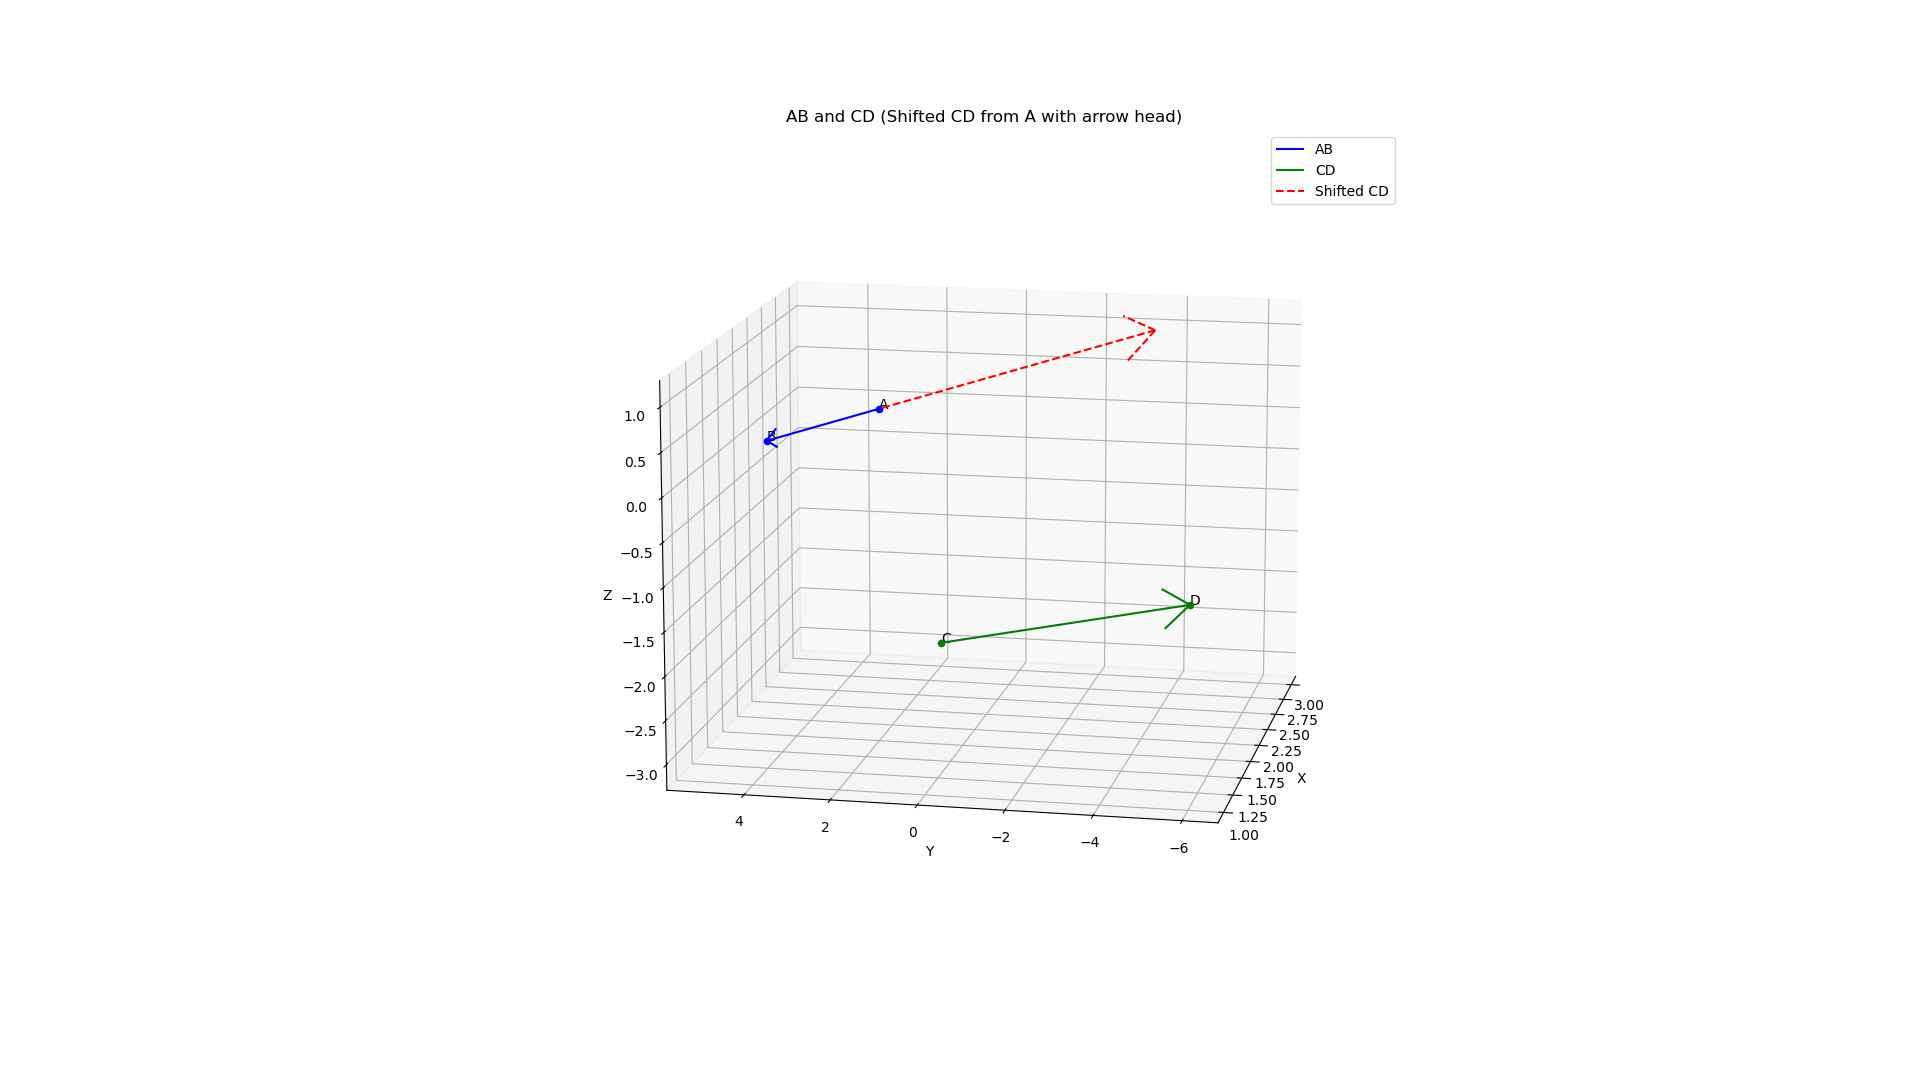
\includegraphics[width=1\columnwidth]{Figs/plot3_1.png}
    \caption{}
    \label{fig:placeholder}
\end{figure}

\textbf{NOTE:} Parallel vectors are collinear.

\end{document}
